% !TeX program = xelatex
% !TeX encoding = UTF-8
\documentclass{MathorCupmodeling}
\let\kaishu\relax
\newCJKfontfamily\kaishu{KaiTi}[AutoFakeBold] %use fake KaiTi
\usepackage{zhlipsum,mwe}%use random characters
\usepackage{mathtools}%use mathtools
\usepackage{amsmath}
\usepackage{siunitx}
\usepackage{graphicx}
\usepackage{enumitem}
\setlist{nosep}

\begin{document}
\begin{center}
{\Large 物理模型和状态空间公式推导部分}

\end{center}
    \newpage

%-------------------------------------------------------------------
为了建立物理模型,现有如下假设:

1、摆杆质量均匀,质心位于其几何中心处

2、忽略除b以外的所有摩擦力


如图\cref{小车受力分析}对小车进行受力分析,以摆杆和小车交点为原点,以水平向右和竖直向下为正方向建立坐标系,沿$x$轴有牛顿第二定律

\begin{figure}[hbpt]
\centering
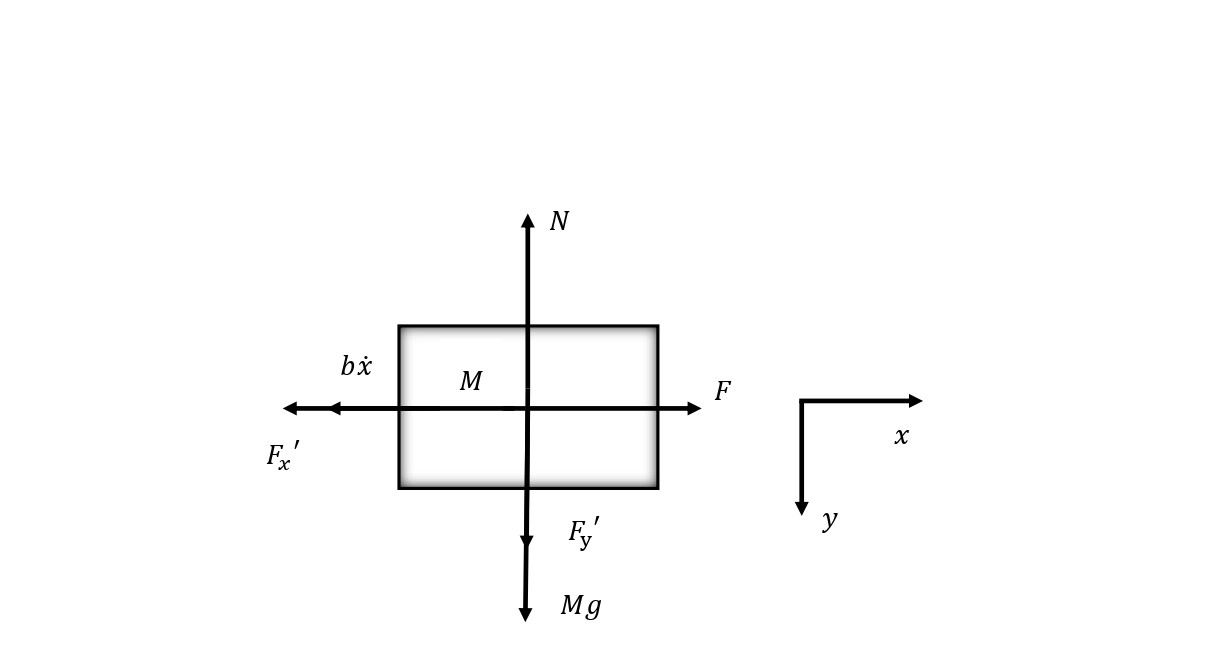
\includegraphics[width=12cm]{小车受力分析.jpg}
\caption{小车受力分析}\label{小车受力分析}
\end{figure}


\begin{equation}
F-b\dot x-N_x^{'}=M\ddot x
\end{equation}

如图\cref{摆杆受力分析}对摆杆进行受力分析,沿$x,y$轴有牛顿第二定律和沿$\theta$向动量矩定理

\begin{figure}[hbpt]
\centering
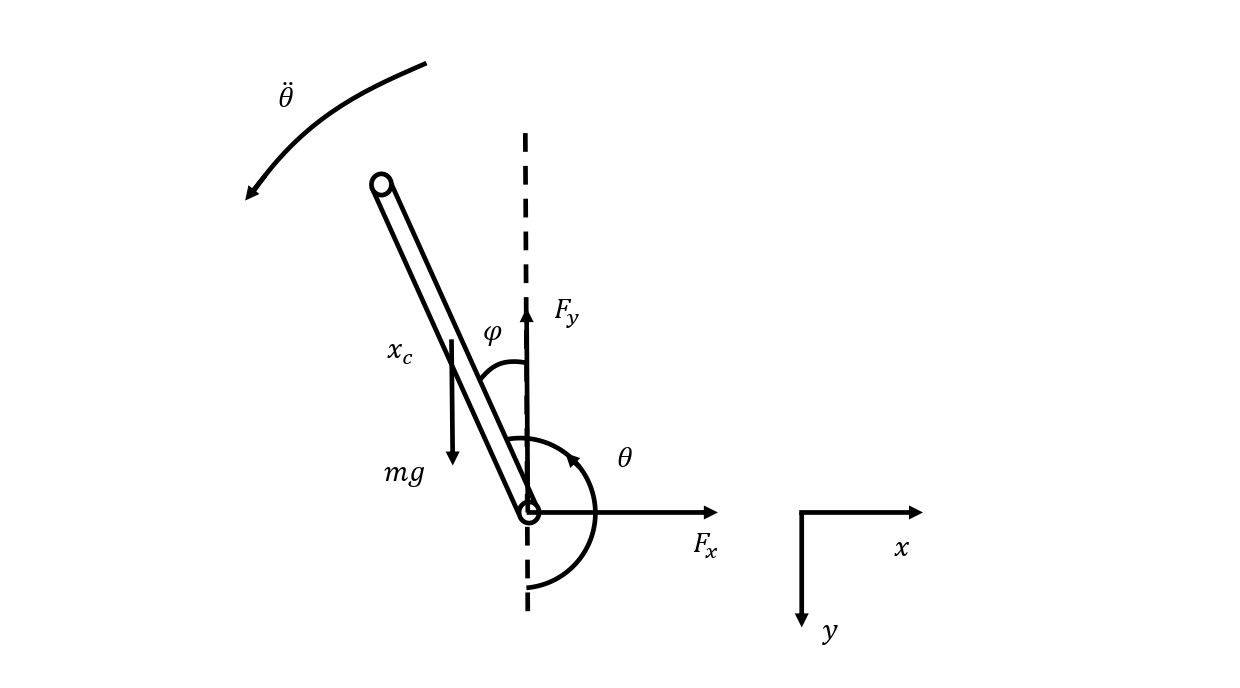
\includegraphics[width=12cm]{摆杆受力分析.jpg}
\caption{摆杆受力分析}\label{摆杆受力分析}
\end{figure}

摆杆质心$c$点
	
\begin{equation}
\begin{aligned}
x_c&=x+lsin\theta\\
y_c&=lcos\theta\\
\end{aligned}
\end{equation}

求导可得质心加速度

\begin{equation}
\begin{aligned}
\ddot x_c&=\ddot x+l\ddot{\theta}cos\theta-l\dot{\theta}^2sin\theta\\
\ddot y_c&=-l\ddot{\theta}sin\theta-l\dot{\theta}^2cos\theta\\
\end{aligned}
\end{equation}
\begin{equation}
\begin{aligned}
&N_y-mg=-m\ddot y_c\\
&N_x=m\ddot x_c\\
&N_ylsin\varphi+N_xlcos\varphi=I\ddot{\varphi}\\
\end{aligned}
\end{equation}

应用小量近似$sinx\doteq x$,$cosx=1-\frac{x^2}{2}$以及$\theta=\varphi+\pi$这个关系整理以上各式,可得倒立摆系统物理方程组

\begin{equation}
\begin{aligned}
&F=(M+m)\ddot x-ml\ddot{\varphi}+b\dot x\\
&(I+ml^2)\ddot{\varphi}=ml\ddot x+mgl\varphi\\
\end{aligned}
\end{equation}

拉氏变换可得

\begin{equation}
\begin{aligned}
&(M+m)X(s)s^2+bX(s)s-ml\varphi(s)s^2=F(s)\\
&(I+ml^2)\varphi(s)s^2-mgl\varphi((s)=mlX(s)s^2\\
\end{aligned}
\end{equation}

注意到小车加速度$A(s)=X(s)s^2$

可得从小车角速度输入到摆杆角度输出的传递函数

\begin{equation}
\frac{\varphi(s)}{A(s)}=\frac{ml}{(I+ml^2)s^2-mgl}
\end{equation}

进一步整理,可以得到力输入到摆杆角度和小车位移的传递函数

\begin{equation}
\begin{aligned}
&\frac{\varphi(s)}{F(s)}=\frac{mls^2}{[(I+ml^2)(M+m)-m^2l^2]s^4+b(I+ml^2)s^3-(M+m)mgls^2-bmgls}\\
&\frac{X(s)}{F(s)}=\frac{(I+ml^2)s^2-mgl}{[(I+ml^2)(M+m)-m^2l^2]s^4+b(I+ml^2)s^3-(M+m)mgls^2-bmgls}
\end{aligned}
\end{equation}

将物理方程组进行等价变形,可以得到

\begin{equation}
\begin{aligned}
&\ddot x=-\frac{bI+bml^2}{\Delta}\dot x+\frac{m^2gl^2}{\Delta}\varphi+\frac{I+ml^2}{\Delta}F\\
&\ddot{\varphi}=\frac{-mlb}{\Delta}\dot x+\frac{mg(M+m)l}{\Delta}\varphi+\frac{ml}{\Delta}F\\
\end{aligned}
\end{equation}

其中,$\Delta=I(M+m)+Mml^2$.

基于此,取$z_1=x,z_2=\dot x,z_3=\varphi,z_4=\dot{\varphi}$为状态空间变量,以力$F$作为输入$u$,建立状态空间矩阵

\begin{equation}
\begin{aligned}
&\begin{bmatrix}
\dot x\\
\ddot x\\
\dot{\varphi}\\
\ddot{\varphi}\\
\end{bmatrix}
=
\begin{bmatrix}
0 & 1 & 0 & 0\\
0 & -\frac{bI+bml^2}{\Delta} & \frac{m^2gl^2}{\Delta} & 0\\
0 & 0 & 0 & 1\\
0 & \frac{-mlb}{\Delta} & \frac{mg(M+m)l}{\Delta} & 0\\
\end{bmatrix}
\begin{bmatrix}
x\\
\dot x\\
\varphi\\
\dot{\varphi}\\
\end{bmatrix}
+
\begin{bmatrix}
0\\
\frac{I+ml^2}{\Delta}\\
0\\
\frac{ml}{\Delta}\\
\end{bmatrix}
u\\
&\begin{bmatrix}
x\\
\varphi\\
\end{bmatrix}
=
\begin{bmatrix}
1 &0 &0 &0\\
0 &0 &1 &0\\
\end{bmatrix}
\begin{bmatrix}
x\\
\dot x\\
\varphi\\
\dot{\varphi}\\
\end{bmatrix}
+
\begin{bmatrix}
0\\
0\\
\end{bmatrix}
u\\
\end{aligned}
\end{equation}

注意到该状态空间矩阵较为复杂,若取小车加速度作为输入$u^{'}$,可以简化该状态空间矩阵

根据转动惯量的定义式,并认为摆件质地均匀,有下式

\begin{equation}
I=\frac{1}{12}m(2l)^2
\end{equation}

带入整理,得

\begin{equation}
\ddot \varphi=\frac{3g}{4l}+\frac{3}{4l}\ddot x
\end{equation}

则可得较为简单的状态空间矩阵

\begin{equation}
\begin{aligned}
&\begin{bmatrix}
\dot x\\
\ddot x\\
\dot{\varphi}\\
\ddot{\varphi}\\
\end{bmatrix}
=
\begin{bmatrix}
0 & 1 & 0 & 0\\
0 & 0 & 0 & 0\\
0 & 0 & 0 & 1\\
0 & 0 & \frac{3g}{4l} & 0\\
\end{bmatrix}
\begin{bmatrix}
x\\
\dot x\\
\varphi\\
\dot{\varphi}\\
\end{bmatrix}
+
\begin{bmatrix}
0\\
1\\
0\\
\frac{3}{4l}\\
\end{bmatrix}
u'\\
&\begin{bmatrix}
x\\
\varphi\\
\end{bmatrix}
=
\begin{bmatrix}
1 &0 &0 &0\\
0 &0 &1 &0\\
\end{bmatrix}
\begin{bmatrix}
x\\
\dot x\\
\varphi\\
\dot{\varphi}\\
\end{bmatrix}
+
\begin{bmatrix}
0\\
0\\
\end{bmatrix}
u^{'}\\
\end{aligned}
\end{equation}

代入数据可得

\begin{equation}
\begin{aligned}
&\begin{bmatrix}
\dot x\\
\ddot x\\
\dot{\varphi}\\
\ddot{\varphi}\\
\end{bmatrix}
=
\begin{bmatrix}
0 & 1 & 0 & 0\\
0 & 0 & 0 & 0\\
0 & 0 & 0 & 1\\
0 & 0 & 29.4 & 0\\
\end{bmatrix}
\begin{bmatrix}
x\\
\dot x\\
\varphi\\
\dot{\varphi}\\
\end{bmatrix}
+
\begin{bmatrix}
0\\
1\\
0\\
3\\
\end{bmatrix}
u'\\
&\begin{bmatrix}
x\\
\varphi\\
\end{bmatrix}
=
\begin{bmatrix}
1 &0 &0 &0\\
0 &0 &1 &0\\
\end{bmatrix}
\begin{bmatrix}
x\\
\dot x\\
\varphi\\
\dot{\varphi}\\
\end{bmatrix}
+
\begin{bmatrix}
0\\
0\\
\end{bmatrix}
u^{'}\\
\end{aligned}
\end{equation}

\end{document}